% Use document class "aletter.cls" (for letters):
\documentclass[11pt, oneside]{essay}

% ISO 8859-1 character encoding is assumed
\usepackage[finnish, english]{babel}
\usepackage[latin1]{inputenc}
\usepackage[T1]{fontenc}
\usepackage{natbib}
\usepackage{color}
\usepackage{amsmath, amssymb}
\usepackage{graphicx} % more modern
\usepackage[nottoc,numbib]{tocbibind}

% shortcuts for math
\newcommand{\hess}{\mathbf{H}}
\newcommand{\jacob}{\mathbf{J}}
\newcommand{\params}{\mathbf{\theta}}
\newcommand{\cost}{\mathcal{L}}
\newcommand{\lout}{\mathbf{r}}
\newcommand{\louti}{r}
\newcommand{\outi}{y}
\newcommand{\out}{\mathbf{y}}
\newcommand{\gauss}{\mathbf{G_N}}
\newcommand{\eye}{\mathbf{I}}
\newcommand{\softmax}{\text{softmax}}
\newcommand{\targ}{\mathbf{t}}
\newcommand{\metric}{\mathbf{G}}
\newcommand{\sample}{\mathbf{z}}

\newcommand{\bmx}[0]{\begin{bmatrix}}
\newcommand{\emx}[0]{\end{bmatrix}}
\newcommand{\qt}[1]{\left<#1\right>}
\newcommand{\qexp}[1]{\left<#1\right>}
\newcommand{\qlay}[1]{\left[#1\right]}
\newcommand{\vect}[1]{\mathbf{#1}}
\newcommand{\vects}[1]{\boldsymbol{#1}}
\newcommand{\matr}[1]{\mathbf{#1}}
\newcommand{\var}[0]{\operatorname{Var}}
\newcommand{\cov}[0]{\operatorname{Cov}}
\newcommand{\diag}[0]{\operatorname{diag}}
\newcommand{\matrs}[1]{\boldsymbol{#1}}
\newcommand{\va}[0]{\vect{a}}
\newcommand{\vb}[0]{\vect{b}}
\newcommand{\vc}[0]{\vect{c}}
\newcommand{\vh}[0]{\vect{h}}
\newcommand{\vv}[0]{\vect{v}}
\newcommand{\vx}[0]{\vect{x}}
\newcommand{\vw}[0]{\vect{w}}
\newcommand{\vs}[0]{\vect{s}}
\newcommand{\vf}[0]{\vect{f}}
\newcommand{\vy}[0]{\vect{y}}
\newcommand{\vg}[0]{\vect{g}}
\newcommand{\vm}[0]{\vect{m}}
\newcommand{\vu}[0]{\vect{u}}
\newcommand{\vt}[0]{\vect{t}}
\newcommand{\vz}[0]{\vect{z}}
\newcommand{\vL}[0]{\vect{L}}
\newcommand{\mW}[0]{\matr{W}}
\newcommand{\mG}[0]{\matr{G}}
\newcommand{\mX}[0]{\matr{X}}
\newcommand{\mQ}[0]{\matr{Q}}
\newcommand{\mU}[0]{\matr{U}}
\newcommand{\mV}[0]{\matr{V}}
\newcommand{\mA}{\matr{A}}
\newcommand{\mC}{\matr{C}}
\newcommand{\mD}{\matr{D}}
\newcommand{\mS}{\matr{S}}
\newcommand{\mI}{\matr{I}}
\newcommand{\td}[0]{\text{d}}
\newcommand{\vsig}[0]{\vects{\sigma}}
\newcommand{\valpha}[0]{\vects{\alpha}}
\newcommand{\vmu}[0]{\vects{\mu}}
\newcommand{\vzero}[0]{\vect{0}}
%\newcommand{\tf}[0]{\text{f}}
\newcommand{\tf}[0]{\text{m}}
\newcommand{\tdf}[0]{\text{dm}}
\newcommand{\TT}[0]{{\vects{\theta}}}
\newcommand{\grad}[0]{\nabla}
\newcommand{\alert}[1]{\textcolor{red}{#1}}
\newcommand{\N}[0]{\mathcal{N}}
\newcommand{\LL}[0]{\mathcal{L}}
\newcommand{\HH}[0]{\mathcal{H}}
\newcommand{\RR}[0]{\mathbb{R}}
\newcommand{\Scal}[0]{\mathcal{S}}
\newcommand{\sigmoid}{\sigma}
\newcommand{\E}[0]{\mathbb{E}}
\newcommand{\enabla}[0]{\ensuremath{%
    \overset{\raisebox{-0.3ex}[0.5ex][0ex]{%
    \ensuremath{\scriptscriptstyle e}}}{\nabla}}}
\newcommand{\enhnabla}[0]{\nabla_{\hspace{-0.5mm}e}\,}
\newcommand{\tred}[1]{\textcolor{red}{#1}}
\newcommand{\todo}[1]{{\Large\textcolor{red}{#1}}}

\DeclareMathOperator*{\argmin}{arg\,min}
\DeclareMathOperator*{\argmax}{arg\,max}

\title{Deep Learning for Statistical Machine Translation}
\author{Kyunghyun Cho\thanks{Department of Information and
    Computer Science, School of Science, Aalto University,
             Finland}}

\begin{document}

\vspace{20mm}

\maketitle

\tableofcontents

\vfill

\newpage

\section{Research Plan: Goals, Hosting Institution and Schedule}

Lately deep neural networks have shown remarkable
performances in various machine learning tasks. They
include\footnote{For a more comprehensive list, see, for
instance, \citep{Bengio2013pami}.}, but are not
limited to, speech recognition \citep[see,
e.g.,][]{Hinton2012sp,Dahl2012} and large-scale object
recognition \citep[see, e.g.,][]{Krizhevsky2012,Hinton2012}
as well as natural language processing \citep[see,
e.g.,][]{Socher2011}. In these cases, deep neural networks
were able to outperform the conventional models and
algorithms significantly. The whole field, thanks to the recent
surge of its popularity, has come to be called \textit{deep
    learning}.\footnote{MIT Technological Review selected deep
learning whose main focus is on deep neural networks as one of the ten breakthrough technologies in
2013:
http://www.technologyreview.com/featuredstory/513696/deep-learning/
}

Based on these advances in academic research, deep neural
networks have rapidly found their way into commercial use
through companies such as Google, Microsoft and Apple.  For
instance, Google Goggles\footnote{
http://www.google.fi/mobile/goggles/} uses a deep belief
network in
production.\footnote{See the invited talk \textit{Machine
Learning in Google Goggles} by Hartmut Neven at the
International Conference on Machine Learning 2011:
http://techtalks.tv/talks/machine-learning-in-google-goggles/54457/}
Microsoft has replaced the existing speech recognition
algorithm based on Gaussian mixtures with one based on deep
neural networks \citep{Deng2013}. Furthermore, the voice
assistance feature of Apple's iPhone, called Siri, as well
as Google's Street View are also known to utilize deep
neural networks.\footnote{See the article \textit{Scientists
See Promise in Deep-Learning Programs} by John Markoff
featured in the New York Times on 23 November 2012: \\
http://www.nytimes.com/2012/11/24/science/scientists-see-advances-in-deep-learning-a-part-of-artificial-intelligence.html
}

One important lesson from these recent breakthroughs and rapid
adoptions of deep learning by the industry is that all components
of a deep learning, or machine learning, system should be tuned
jointly to optimize for the overall performance of the system. In
object recognition, for instance, it has been usual, before the
breakthrough made by deep learning, to build a system that
consists of separate stages of feature extraction and
classification/recognition. Often, the feature extraction was
done by engineering a set of features using the domain knowledge
of each task, without directly optimizing the final recognition
performance. Only then with the extracted features, the
recognizer was trained to maximize the recognition performance.
On the other hand, the recently introduced deep neural networks,
which outperformed most of the conventional approaches for
object recognition, combines both the stages in a single
architecture and jointly optimizes them together to maximize
the final performance.

Until now, the application that has benefited most from adopting
the approach of deep learning has been the task of object/speech
recognition. Recently, however, more and more applications are
emerging and being found to benefit from employing deep neural
networks. Deep neural networks have been applied to, for
instance, bioinformatics \citep[see, e.g.,][]{Lena2012}, human
gesture recognition \citep[see, e.g.,][]{Cho2014} and language
modeling \citep[see, e.g.,][]{Mikolov2010,Bengio2003}.

In my post-doctoral research years, I aim to further push the
boundary of deep learning by proposing and studying a novel
approach to solving the task of statistical machine translation
(SMT) using deep neural networks. The conventional phrase-based
SMT system \citep{Koehn2003,Marcu2002} consists of multiple
stages that are often hand-engineered and separately tuned, just
like the conventional object recognition system used to have at
least two separate stages of feature extraction and recognition.
\textbf{The goal of my post-doctoral research is to replace
this conventional SMT system with a single model built with
advanced neural networks, where the whole system is jointly
tuned to maximize the final translation performance}.

In the remainder of this section, I will first justify the choice
of the Machine Learning Lab at the University of Montreal as an
ideal place for conducting research on applying deep learning to
the task of statistical machine translation. Then, a detailed
schedule of my post-doctoral years will be given.

After this section, I will describe some background materials on
statistical machine translation (SMT) and how neural networks so
far have been applied to the existing SMT systems in
Sec.~\ref{sec:smt}. Based on this description, a novel approach to
the SMT system based \textit{purely} on deep neural networks will
be proposed in Sec.~\ref{sec:new_approach}.  Benefits from
implementing this novel approach will be discussed, and
potential challenges that need to be addressed during my
post-doctoral research period will be described.

\subsection{Machine Learning Lab at University of Montreal}

Here let me briefly explain why the Machine Learning Lab
(Laboratoire d'Informatique des Syst\`emes Adaptifs, LISA) at the
University Montreal is an ideal place to conduct my research on
applying deep learning to statistical machine translation (SMT).

The LISA lab is the leading research lab led by Prof. Yoshua
Bengio who is one of the leading researchers in the field of
\textit{deep learning}. He has started his research on neural
networks already from 1980's and has continued working on deep
neural networks ever since. The LISA lab was one of three
research groups who proposed the method of layer-wise pretraining
for deep neural networks in 2006 and 2007 \citep{Bengio2007nips},
which led to the so-called second neural network renaissance
\citep{Schmidhuber2011}.

As far as statistical machine translation (SMT) is concerned, Prof.
Bengio is one of the pioneers who proposed to use a neural
network to learn the language model (See Sec.~\ref{sec:nnlm}). In
2003, Prof. Bengio proposed the first language modeling technique
based on feedforward neural network \citep{Bengio2003} and in
2006 showed that it is possible to improve the existing speech
recognition system by using this approach \citep{Bengio2006},
together with Prof.  Holger Schwenk whose lab I am
planning to make a visit to during my post-doctoral
period.

There are a number of active researchers in the LISA lab who have
internationally-renowned expertise in building and training
sophisticated neural networks, especially recurrent neural
networks which will be the crucial component of the novel
approach I am planning to pursue (See
Sec.~\ref{sec:autoencoder}). Razvan Pascanu, M.Sc. has recently
shown that it is possible to train a deep recurrent neural
network to model long-term dependencies in long temporal
sequences \citep{Pascanu2013}. Also, Caglar Gulcehre, M.Sc. who
has deep knowledge on the difficulties of optimization problems
in machine learning \citep{Gulcehre2013a} began
collaborating with Pascanu and me on recurrent neural networks
recently with already some successful publication
\citep{Pascanu2013}. Prof. Bengio has also been active in
research on recurrent neural networks \citep[see,
e.g.,][]{Bengio2013rec}, where recurrent
neural networks have been his main research topic
already from early 1990's \citep[see,
e.g.,][]{Bengio1994}.

The LISA lab is actively collaborating with external researchers.
The external collaborators\footnote{The list of external
collaborators as well as the members of the LISA lab may be
found at http://lisa.iro.umontreal.ca/who\_en.html.}
include, for instance, Prof. Hal Daume III of the
University of Maryland who is the internationally
renowned expert on statistical natural language
processing which is at the core of statistical machine
translation. Dr. L\'eon Bottou of Microsoft Research has
worked on applying advanced machine learning techniques
to natural language processing.  Collaborations with
these external researchers will be invaluable to my
post-doctoral research.


\subsection{Schedule}

I plan to conduct my post-doctoral research at the Machine
Learning Lab (LISA), University of Montreal to last two years
starting from April, 2014 after the planned defense of my Ph.D.
Dissertation early March, 2015. 

\textbf{Apr., 2014--Dec. 2014}: During the three quarters of the first
year I will concentrate on exploring various neural network
architectures to assess the feasibility of each design for the
task of statistical machine translation (SMT). The work will mainly
focus on using recurrent neural networks, but will not entirely
be restricted to them. During this period I will focus more on
developing novel architectures as well as designing a novel
learning algorithm, which will make experiments run on a rather
limited set of data such as the news commentary corpus from the
Workshop on Machine Translation.

I plan to report on findings from implementing these novel
architectures to a number of conferences related to machine
learning and natural language processing such as the
international conference on machine learning (ICML), advances in
neural information processing (NIPS) and the annual meeting of
the association for computational linguistics (ACL). By attending
these conferences and reporting my own work, potential for future
collaboration, possibly continuing even after the post-doctoral
period, will greatly increase.

\textbf{Jan. 2015--Dec. 2015}: In 2015 I plan to implement the
fully functional neural network that will replace the existing
SMT system. In order to train this fully functional SMT system
based on neural networks it is important to train the neural
network with large datasets such as Europarl \citep{Koehn2005}
and MultiUN \citep{Eisele2010} corpora. The scalability will
inevitably become a big issue when training these large neural
networks with even larger training corpora, which will be the
central research theme of this period.

Solving the issue of scalability will require work in both the
design of the system as well as learning algorithms. Especially,
I will focus my effort on building a scalable, parallel learning
algorithm for recurrent neural networks that may be used to
efficiently train the whole, proposed SMT system. 

Again, research findings from this period will be reported to the
research community, both deep learning and natural language
processing, through a number of conference. Unlike the previous
period, most of the findings will, however, be reported to
conferences more focused on natural language processing and
statistical machine translation during this period. Those
conferences include ACL, the conference of the European chapter
of the association for computational linguistics (EACL), the
international conference on computational linguistics (COLING)
and empirical methods in natural language processing (EMNLP). 

\textbf{Jan. 2016--Mar. 2016}: I will mainly concentrate on
making the underlying code of the implemented SMT system public.
This will allow not only researchers but also practitioners in
statistical machine translation and natural language processing
to have access to the latest technology. Also, I will start
collaborating with researchers who have expertise in
non-Indo-European languages such as Finnish and Korean to extend
the novel SMT system to machine translation based on sub-word
units such as morphemes \citep[see, e.g.,][]{Creutz2007}.

\subsection{Outline}

In the remainder of this document, I describe in detail
statistical machine translation (SMT) and how neural networks
have been applied to the conventional SMT system in
Sec.~\ref{sec:smt}. Specifically, in Sec.~\ref{sec:smt-basic},
the basic principles behind SMT are introduced, where a
general framework on SMT is divided into the
inverse-translation model and the language model. 
Sec.~\ref{sec:nntm}--\ref{sec:nnlm} introduce earlier works on
using neural networks for these two components of the SMT system. 

In Sec.~\ref{sec:new_approach}, I propose and introduce a novel
approach to building a SMT system using deep neural networks.  I
begin by giving out a generative view of natural languages in
Sec.~\ref{sec:genlm} and continue on to introducing the concepts
of encoding and decoding from this generative perspective. The
novel architecture based on this generative perspective is
proposed and described in Sec.~\ref{sec:autoencoder}. The last
section~\ref{sec:challenges} lists challenges that need to be
addressed in order to implement the proposed SMT system, and they
will be the central problems during my post-doctoral period.











\section{Neural Networks in Statistical Machine Translation}
\label{sec:smt}

In this section, I describe how neural networks may be applied to
the task of statistical machine translation (SMT) by first
starting with a probabilistic framework behind SMT. Then, I
introduce some earlier works that have applied neural networks to
the task of language modeling which is an important component of
the SMT system.

\subsection{Probabilistic Framework behind Statistical Machine
Translation}
\label{sec:smt-basic}

A statistical machine translation (SMT) system may be described
in the following, single equation:
\begin{align}
    \label{eq:smt_fund}
    \vt^* = \argmax_{\vt} p(\vt \mid \vs),
\end{align}
where $\vs$ and $\vt$ are respectively the source and target
sentences, and $\vt^*$ is the most likely target sentence which
corresponds to the correct translated sentence under the SMT
system. It is common to decompose this equation into an
inverse-translation probability and a language modeling using
Bayes' rule such that
\begin{align}
    \label{eq:smt}
    \vt^* = \argmax_{\vt} p(\vt \mid \vs) 
    = \argmax_{\vt} p(\vs \mid \vt) p(\vt),
\end{align}
where $p(\vs \mid \vt)$ is the inverse-translation probability
and $p(\vt)$ is the language model of the target language
\citep{Koehn2010}.

In this probabilistic framework, the task of SMT is broken down
into two parts; (1) inference and (2) learning. 

\textit{Inference} corresponds to the actual task of \textit{translating} a
given sentence $\vs$ into a foreign sentence $\vt^*$. The best
target sentence $\vt^*$ can be found by search for a pair
$\left(\vs, \vt\right)$ that gives the highest
\textit{probability} $p(\vt \mid \vs)$ given by the model in
Eq.~\eqref{eq:smt}.

\textit{Learning} is used to \textit{estimate} $p(\vt \mid \vs)$
from data.  Often, one uses separate models for the
inverse-translation model $p(\vs \mid \vt)$ and the language
model $p(\vt)$ and combines them as a log-linear model:
\begin{align}
    \label{eq:loglinear}
    p(\vt \mid \vs) \propto \exp\left\{ \omega_0 \log p(\vs \mid
    \vt) + \omega_1 \log p(\vt) \right\}, 
\end{align}
where $\omega_0$ and $\omega_1$ are the weights for the
inverse-translation model and the language model, respectively.
In this case, learning may be decomposed into learning the
inverse-translation model, learning the language model and
learning their weights.

This approach based on the log-linear model in
Eq.~\eqref{eq:loglinear} opens the possibility of integrating
more features that are neither the inverse-translation model nor
the language model. Given a pair of source and target sentences,
one may use any other model or mechanism to compute a
\textit{feature} that may be integrated into the log-linear
model. Mathematically, this corresponds to generalizing $p(\vt
\mid \vs)$ in Eq.~\eqref{eq:loglinear} into
\begin{align}
\label{eq:loglinear_general}
    p(\vt \mid \vs) \propto \exp\left\{  
    \sum_{m=1}^M \omega_m f_m(\vs, \vt)
    \right\}, 
\end{align}
where $f_m$ and $\omega_m$ are the $m$-th feature function and
its corresponding weight, respectively. The $M$ features include
the inverse-translation model and the language modeling as well
as any other user-defined features.

In the remainder of this section, I introduce a number of
recently proposed approaches for modeling the
inverse-translation model and the language model.

\subsection{Neural Networks for Inverse-Translation Model}
\label{sec:nntm}

The inverse-translation model in Eq.~\eqref{eq:loglinear} is conventionally
implemented by a phrase-based approach \citep[see,
e.g.,][]{Koehn2003,Marcu2002}.  In the phrase-based approach, the
inverse-translation probability is decomposed into the
probabilities of short phrases:
\begin{align}
\label{eq:phrase_decomp}
    p(\vs \mid \vt) = \frac{1}{Z(\vt)} \prod_{i=1}^{I} \phi(\vs_i \mid \vt_i) d(a_i -
    b_i -1),
\end{align}
where $phi(\vs_i \mid \vt_i)$ and $d(a_i - b_i - 1)$ are the
phrase translation probability and the reordering weight based on
the start and the end of the $i$-th phrase of the source sentence
$\vs_i$. $Z(\vt)$ is a normalization constant that makes the
probabilities sum up to one. Here, it is assumed that the
sentence is decomposed into $I$ phrases. Learning this model,
thus, consists of (1) learning the phrase translation model and
(2) deciding/learning the reordering model.  

Traditionally it is usual to implement the phrase translation
model with a phrase pair table. The phrase pair table contains a
list of all possible pairs of source and target phrases from data
and their corresponding (smoothed) frequencies \citep[see,
e.g.,][]{Koehn2003,Koehn2010}. 

Neural networks, however, can be used to replace this
frequency-based table. In the remainder of this section, I
describe two approaches to the inverse-translation model based on
neural networks.

\subsubsection{Feedforward Neural Networks}

In the phrase-based translation, it is often the case that most
of the phrases, both source and target, are quite short (often,
        less than $8$ words). Hence, it is possible to directly
model the mapping from a source phrase to the corresponding
target phrase assuming the maximum number of words per phrase.
Learning this mapping corresponds to modeling the phrase
translation probability $p(\vs_i \mid \vt_i)$ which is equivalent to
a single term $\phi(s_i \mid t_i)$ in
Eq.~\eqref{eq:phrase_decomp}.

In \citep{Schwenk2012,Son2012}, an approach of learning the phrase
pair table directly using a feedforward neural network was
proposed and discussed in detail. \citet{Schwenk2012} assumes that
each phrase consists of at most seven words and models the phrase
translation probability by
\begin{align}
\label{eq:fftm}
p(\vs_i \mid \vt_i) = \prod_{j=1}^M p(s_i^j \mid \vt_i) 
                     = \prod_{j=1}^M \softmax\left( \mW_j^\top
                             \phi \left( \sum_{k=1}^M \mU_k^\top
                                 \mC^\top t_i^k  \right) \right),
\end{align}
where $\mW_j$ is the projection matrix for the $j$-th word of the
source phrase $\vs_i$, and $\mU_k$ are the projection
matrix for the embedding of the $k$-th word of the target phrase
$\vt_i$. The embedding of each target word is defined as a row of
the common embedding matrix $\mC$. $\phi$ is an element-wise
nonlinear function used for computing the hidden representation
of the target phrase. Each word $s_i^j$ or $t_i^j$ is represented
as a one-hot vector.

One important advantage of this inverse-translation model based
on feedforward neural networks (FFTM) in Eq.~\eqref{eq:fftm} is
that this model naturally generalizes to an unseen pair of source
and target phrases. In the case of the table-based phrase
translation model, one has to opt for heuristics such as
smoothing techniques to be able to cope with those pairs that
have \textit{zero} probability according to data. However, the
FFTM which first projects the input phrase into a continuous
space embedding automatically interpolates/extrapolates to unseen
pairs.


\subsubsection{Bilingual Word Embeddings}
\label{sec:biembed}

It should be noticed from the previous section on the
inverse-translation model based on feedforward neural networks
(FFTM) as well as the language modeling based on neural networks
which will be discussed later in this section, that most neural
networks-based approaches learn a continuous-space word embedding
($\mC$ in Eq.~\eqref{eq:fftm}). The embedding maps each word,
often represented by a one-hot vector, to a fixed-length
vector (a row of $\mC$) in a continuous space.  In this case,
one can readily utilize the word embeddings (regardless of how
they were learned) of source and target languages to
estimate the probability of a pair of phrases. 

\citet{Zou2013} proposed to learn the word embeddings of two
languages (Chinese and English) by regularizing the linearly
transformed embeddings of those languages $\mA_{c\to e} \mC_c$
and $\mA_{e\to c} \mC_e$ to be close to each other. The
regularization term, called the translation equivalence
objective, is defined as
\begin{align}
\label{eq:TEO}
\left\| \mC_e - \mA_{c \to e} \mC_c \right\|^2_{\text{F}} + 
\lambda \left\| \mC_c - \mA_{e \to c} \mC_e \right\|^2_{\text{F}},
\end{align}
where $\lambda$ is a constant that balances the two terms.

Once the \textit{compatible} word embeddings are learned by, for
instance, training FFTM in Eq.~\eqref{eq:fftm} together with the
above regularization term in Eq.~\eqref{eq:TEO}, \citet{Zou2013}
proposed to compute the embedding of a phrase by averaging the
embeddings of the words in the phrase. Then, the phrase
translation probability, or score, is defined by the distance
between the embeddings of source and target phrases:
\begin{align*}
p(\vs_i \mid \vt_i) \propto \angle\left( \vc_s, \vc_t
        \right),
\end{align*}
where $\vc_s$ and $\vc_t$ are respectively the embeddings of the
source and target phrases, and the function $\angle(\cdot,\cdot)$
computes the cosine distance between those embeddings.

As was the case with the FFTM, this approach of learning
bilingual word embeddings can generalize to unseen pairs of
phrases, unlike the table-based inverse-translation model.












\subsection{Neural Networks for Language Modeling}
\label{sec:nnlm}

There are rather diverse approaches to learning the language
model. The most naive approach, called $n$-gram language model,
assumes $n^{\text{th}}$-order Markov property and decomposes the
language model $p(\vt)$ into
\begin{align}
    \label{eq:ngram}
    p(\vt) = \prod_{l=1}^L p(t_l \mid t_{l-n}, \dots, t_{l-1}),
\end{align}
where each $t_l$ corresponds to the $l$-th word in a sentence
$\vt$. Then, each $n$-gram probability $p(t_l \mid t_{l-n},
\dots, t_{l-1})$ can be learned from data by simply counting the
number of occurrences of the $n$-gram. 

This $n$-gram approach is a \textit{discrete}-space approach in
the sense that the $n$-gram model can be effectively represented
by a table with a finite number $O(k^n)$ of entries, where there
are $k$ distinct words/symbols. Unfortunately, this approach is
limited by the fact that as $n$ increase, the number of unseen
$n$-grams increases exponentially, which affects the overall
performance of SMT system relying on this language model badly. 

Alternatively, one may resort to a continuous-space language
model. In this approach, one models each term in
Eq.~\eqref{eq:ngram} with, for instance, a neural network
\citep{Bengio2003}. The neural network trained with data will
then be able to interpolate and extrapolate to generalize to
unseen $n$-grams. Furthermore, one can use a neural network that
does not require the assumption of Markov property, such as
recurrent neural networks (RNN) \citep{Rumelhart1986,Mikolov2010}. 

In this section I describe a number of approaches to
language modeling based on neural networks. This approach based
on neural networks is important, as it will constitute a basis on
which my research goal will be conducted. 

\subsubsection{Feedforward Neural Network}

A neural network can model the $n$-gram model in
Eq.~\eqref{eq:ngram}, by learning a nonlinear mapping from $n$
previous words $\left\{ t_{l-n}, \dots, t_{l-1} \right\}$ to the
$l$-th word $t_l$. \citet{Bengio2003} proposed a feedforward
neural network architecture that subsequently performs (1)
projecting the previous $n$ words into a common continuous-space
representation and (2) combining them to predict the probability
of the next word $t_l$. 

Mathematically, the $n$-gram model using a feedforward neural
network can be written as, for instance, 
\begin{align}
\label{eq:fflm}
    p(t_l =t \mid t_{l-n}, \dots, t_{l-1}) = \softmax
    \left( \mW^\top \tanh\left(\sum_{i=1}^n \mC^\top t_{l-i} +
    \vb\right) +\vc
    \right),
\end{align}
where $\mC$ is the word embedding matrix shared by all $n$
previous words. $\vb$ and $\vc$ are bias vectors, and $\mW$ is
the weight parameter. Each word $t_l$ is represented by a
so-called one-hot vector of which a single element corresponding
to the word is set to $1$ while all other elements are $0$.

\subsubsection{Recurrent Neural Networks}

A recurrent neural network (RNN) is able to simulate a discrete
dynamical system that has an input $\vx_t$, an output $\vy_t$ and
a hidden state $\vh_t$.  The dynamical system is defined by
\begin{align}
    \label{eq:dynamical_system_trans}
    \vh_t &= f_h(\vx_t, \vh_{t-1}) 
    \\
    \label{eq:dynamical_system_out}
    \vy_t &= f_o(\vh_t),
\end{align}
where $f_h$ and $f_o$ are a state transition function and an
output function, respectively. Each function is parameterized by
a set of parameters; $\TT_h$ and $\TT_o$, respectively. 

If an RNN is trained to output, or predict, the input at the next
timestep $t+1$, one may directly use the RNN to learn the
language model $p(\vt)$ in Eq.~\eqref{eq:smt} without the Markov
assumption. This is possible, since the output $\vy_t$ depends on
all previous inputs $\left\{ \vx_1, \dots, \vx_{t-1} \right\}$.

When the language model $p(\vt)$ is decomposed into
\[
    p(\vt) = \prod_{l=1}^L p(t_l \mid t_{l-1}, \dots, t_1),
\]
an RNN can learn this language model by 
\[
    p(t_l \mid t_{l-1}, \dots, t_1) = f_o(f_h(t_{l-1},
    f_h(t_{l-2}, \dots, f_h(t_1, \vzero)))),
\]
which is an unfolded expression of the RNN given in
Eqs.~\eqref{eq:dynamical_system_trans}--\eqref{eq:dynamical_system_out}
\citep{Mikolov2010}.

The transition model in Eq.~\eqref{eq:dynamical_system_trans} is
often implemented as
\begin{align}
\label{eq:rnn_simple_trans}
f_h(\vx_t, \vh_{t-1}) = \tanh\left( \mC^\top \vx_t + \mU^\top
        \vh_{t-1}\right),
\end{align}
where $\mC$ and $\mU$ are the word embedding matrix (as in
Eq.~\eqref{eq:fflm}). 




\section{Statistical Machine Translation based Purely on Neural Networks}
\label{sec:new_approach}

The methods based on neural networks discussed in the previous
section have been found to improve the overall translation
performance. Those approaches, however, constitute only a certain
part of a large statistical machine translation (SMT) system. For
instance, the language model $p(\vt)$ is effectively a single
term in the generalized log-linear model used to score a pair of
source and target sentences in Eq.~\eqref{eq:loglinear_general}.
Also, the inverse-translation models $p(\vs_i \mid \vt_i)$ are
often used to only rescore/rerank the list of candidate phrase
pairs, which again corresponds to another term in the generalized
log-linear model.  A large part of the SMT system, that
especially involves
\textit{generating} a target sentence, still has not benefited
much from nor utilized neural networks. 

Based on these observations that (1) replacing certain components
of the SMT system with neural networks improves the overall
translation performance and that (2) still a large part of the
SMT system does not employ neural networks, in this section, I
propose a novel approach to implementing SMT system purely based
on a neural network that can directly generate multiple, correct
target sentences after understanding the source sentence. This
approach will be the main topic of my research during the
post-doctoral years at the University of Montreal.

\subsection{Generative Model of a Language}
\label{sec:genlm}

Here let me first loosely define a generative model
$\mathcal{M}_t$ that \textit{generates} a language $L_t=\left\{
\vs_1, \vs_2, \dots \right\}$ which is a set of all possible,
grammatically correct sentences. Then, the model $\mathcal{M}_t$
is defined by a set of
discrete \textit{concepts} $C = \left\{ c_1, c_2, ... \right\}$,
the prior distribution $p(c_i)$ and 
a set of the corresponding stochastic processes $P=\left\{
\mathcal{LP}^t_{c_1}, \mathcal{LP}^t_{c_2}, \dots \right\}$.

The model $\mathcal{M}_t$ generates the language $L_t$ by
\begin{enumerate}
\item Pick a concept $c$ from $C$ with a probability $p(c)$.
\item Sample a sentence $\vs$ from $\mathcal{LP}^t_c$, i.e., $\vs \sim
\mathcal{LP}^t_c$.
\end{enumerate}

The concepts in this generative model are \textit{independent} of
an actual language. Linguistic features of the language such as
grammatic structures and vocabularies are encoded in the
conditional stochastic processes. In other words, the concepts
may be shared by multiple languages, while the stochastic
processes that actually generate sentences cannot be.

In this perspective of languages, the task of statistical machine
translation (SMT) corresponds to, first, infer the posterior
distribution of the concept given a source sentence
$p_{\mathcal{M}_s} (c \mid \vs)$, sample a concept $\hat{c}$ from
the posterior distribution and generate a corresponding target
sentence from $\mathcal{LP}^t_{c}$ of the target model
$\mathcal{M}_t$. 

The inference step corresponds to \textit{encoding} a given
source sentence into a concept. The sampling step
\textit{decodes} from the encoded concept a sentence in the
target language. This encoder-decoder perspective makes it easy
for us to design a neural network that can replace the whole
SMT system, which will be described in more detail in the
remainder of this section.

\subsection{Encoder-Decoder Approach using Neural Operators}
\label{sec:autoencoder}

Here I propose a neural network architecture that performs both
\textit{inference} and \textit{generation} in the generative
model of languages described above.  The proposed architecture
consists of an \textit{encoder} and a \textit{decoder} that
respectively infers the most likely concept of a source sentence
and generates a target sentence given the inferred concept.

Let me first define a set of operators that will be used to
construct the proposed neural network architecture
\citep[see, e.g.,][]{Pascanu2013}. 

First, a \textit{plus} operator $\oplus: \RR^d \times \RR^d \to
\RR^d$ is defined. The plus operator accepts two fixed-length
vectors that represent an arbitrary embedding $\vh$ and a word
embedding $\vt$, respectively, and returns the embedding $\vh'$
that summarizes both $\vh$ and $\vt$. Secondly, I define an
\textit{emit} operator $\lhd: \RR^d \times \RR^d \to \RR^d$ that
outputs stochastically the \textit{first} word of a sentence
given the summary of what have been emitted so far $\vh$ and the
concept encoded by a fixed-length vector $\vz$.

A neural network can be designed to mimic the
inference-generation procedure of the SMT system using the
generative models $\mathcal{M}_s$ and $\mathcal{M}_t$ of source
and target languages. 

The inference/encoding step is then implemented as
\begin{align}
\label{eq:encoder}
\vz = (\dots ((\vzero \oplus s_1) \oplus s_2) \oplus s_3) \oplus \dots
\oplus s_L),
\end{align}
where $s_l$ is the $l$-th word of a source sentence $\vs$. The
fixed-length vector $\vz$ which encodes the source sentence then
can be considered a vector representation of the most likely
concept.

Given the concept encoded by $\vz$, a target sentence $\vt$ can
be generated/sampled recursively by, at each timestep,
\begin{align}
\label{eq:decoder}
t_l = \lhd \left(\vh_l, \vz\right), \nonumber\\
\vh_{l+1} = \vh_l \oplus t_l,
\end{align}
where $\vh_0$ is initialized to zeros ($\vzero$). Each step of
this recursion emits a single word and tracks what words have
been emitted so far.

Each operator is implemented by a deep neural network (DNN) which
is known to be able to capture highly nonlinear mapping between
the input and output \citep{Rumelhart1986}. This way of
implementing the plus and emit operators as DNNs results in a
deep recurrent neural network which was proposed recently by
myself together with co-authors in \citep{Pascanu2013}. See
Fig.~\ref{fig:autoencoder} for an illustration of this type of
neural network.


\begin{figure}[t]
\centering
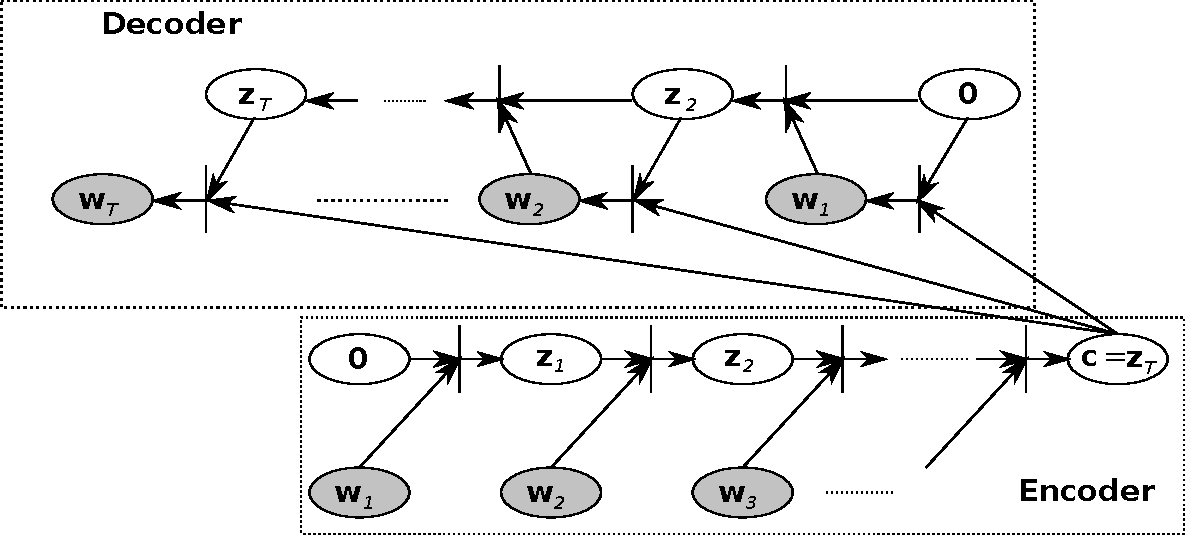
\includegraphics[width=0.8\textwidth]{autoencoder.pdf}
\label{fig:autoencoder}
\caption{An illustration of a neural network that implements the
    encoder and the decoder of a generative model of a language.}
\end{figure}

An important difference of the proposed neural network from the
inference and generation procedures the generative model in
Sec.~\ref{sec:genlm} is that the encoded concept $\vz$ is
\textit{not} stochastic. While the exact probabilistic treatment
would have required that the concept be sampled from the inferred
posterior distribution $p(\vz \mid \vs)$, the neural network
approach directly maps from the source sentence $\vs$ to the
generation probability $p(\vt\mid \vs)$
\textit{deterministically}. This means that the neural network is
trained to effectively marginalize out the concept $\vz$ by
learning $p(\vt \mid \vs)$ directly.

The main advantage of building this type of a neural network  is
that one can readily translate a given sentence in one language
to the other in a single sweep. The encoder will read all symbols
sequentially from the beginning to the end to summarize the
sentence, and the decoder will generate sequentially a list of
symbols that corresponds to the summary encoded by the encoder.
This approach implements the whole SMT system in a single neural
network without any combinatorial search which may become
exponentially expensive due to a large search space (a space of
all possible sentences in a target language).

There are a number of additional advantages from this approach of
replacing the whole SMT system with a single neural network.
First, it becomes more intuitive to extend the system for
multi-lingual translation system. One can simultaneously train
multiple encoders and decoders for more than two languages, while
constraining the summaries of the encoders to be compatible with
each other, which may be implemented similarly to the bilingual
word embeddings described in Sec.~\ref{sec:biembed}. 

Second, the whole system is tuned jointly to optimize for the end
goal of the SMT system which is to maximize the translation
performance. Each component of the conventional SMT system such
as the language model, the inverse-translation model and the
phrase pair table is often tuned separately with its own
objective which is usually not directly related to the
translation performance of the overall SMT system. However, in
this new, proposed approach, the whole system and its
constituents (namely, the encoder and the decoder) are all
together tuned to maximize the actual objective of the system.

Lastly, the proposed approach based purely on neural networks
requires only minimal domain knowledge. Although the name,
\textit{statistical} machine translation, suggests that
the conventional system also focuses more on learning
from data, the conventional SMT system still relies on
domain knowledge about source and target languages
pretty heavily. For instance, the reordering score
$d(a_i -b_i -1)$ from the inverse-translation model in
Eq.~\eqref{eq:phrase_decomp} requires a human designer
to decide on how much and/or what kind of reordering
makes more sense between the target and source
sentences. The proposed system based on neural networks, in
essence, does not require any domain knowledge, though it may be
possible to design a better neural architecture by considering
domain knowledge.


\subsection{Challenges in Encoder-Decoder Approach for
Machine Translation}
\label{sec:challenges}

Although the proposed, novel approach has many advantages over
the conventional statistical machine translation (SMT) system,
many challenges lie ahead before fully implementing the new
system. It will be my main research goal next two years in
the University of Montreal to address these challenges.

First of all, more alternative designs of a neural network must
be investigated. The design proposed earlier in this section is
just one possible design and should not be considered the only
possible design. For instance, a recursive neural network
proposed by \citet{Socher2011} may be used as the encoder instead
\citep{Kalchbrenner2012}. Furthermore, it is possible to combine
undirected graphical models, such as Boltzmann machines
\citep{Ackley1985} or neural autoregressive density estimator
\citep[NADE,][]{Larochelle2011}, with the decoder based on
recurrent neural networks. This may improve the generative
performance of the decoder \citep[see, e.g.,][]{Bengio2013rec}.
This exploration of alternative architectures will be one of the
most important research theme during my post-doctoral years.
      
Secondly, it is not clear if the neural network that
implements the whole SMT system will be easy to train. Until
recently it has been believed by many that it was considered
almost impossible to train a neural
network, not even mentioning how large it is \citep[see,
e.g.,][]{Bengio2009a}. Only recently when it has been found that
deep neural networks can be easily trained by carefully designing
a network \citep[see,
e.g.,][]{Hinton2012sp,Goodfellow2013,Gulcehre2013} and training
the network with recently proposed learning algorithms \citep[see,
e.g.,][]{Martens2012,Hinton2012,Amari1998}. Especially, it has
been long known that training
a recurrent neural network (which is the
main type of networks used in the new approach) is
often more difficult than training a non-recurrent,
feedforward neural network \citep[see,
e.g.,][]{Bengio1994,Sutskever2011,hochreiter1997long}. Therefore,
the foremost challenge to be addressed will be to evaluate
the existing learning algorithms for the novel neural network
architecture and if necessary, to design a new learning
algorithm that will facilitate training it.

The third challenge is the scalability. Considering the highly
complex structure of a language as well as probably even more
complicated relationships among multiple languages, it is clear
that the neural network that implements the proposed approach
must be much larger than ones that have been used, for instance,
for recognizing a fixed set of objects from a still images
\citep[see, e.g.,][]{Krizhevsky2012,Le2012}, though those
neural networks are already large taking multiple gigabytes
of memory only for storing the parameters and more than a
week to train them. For instance, one of the standard datasets
used for training the SMT systems, called Europarl
\citep{Koehn2005}, includes 21 European languages and around 60
million word occurrences for each language. Each language has
more than 50 thousands unique words. Considering that this is
just a single dataset among many others that may need to be used
later, it is not difficult to understand that the scalability
will be an important issue to be addressed.

As this approach is very new in the sense that there has been
essentially no prior work, there will be many challenges that
cannot be expected nor forecastable at the moment. Those
challenges, however difficult they are, will, in addition to the
three challenges discussed here, constitute good research
problems that should and need to be solved during my
post-doctoral years at the University of Montreal.




















%\small
\bibliographystyle{research_plan}
\bibliography{research_plan}





\end{document}
